%
% File naacl2019.tex
%
%% Based on the style files for ACL 2018 and NAACL 2018, which were
%% Based on the style files for ACL-2015, with some improvements
%%  taken from the NAACL-2016 style
%% Based on the style files for ACL-2014, which were, in turn,
%% based on ACL-2013, ACL-2012, ACL-2011, ACL-2010, ACL-IJCNLP-2009,
%% EACL-2009, IJCNLP-2008...
%% Based on the style files for EACL 2006 by 
%%e.agirre@ehu.es or Sergi.Balari@uab.es
%% and that of ACL 08 by Joakim Nivre and Noah Smith

\documentclass[11pt,a4paper, french]{article}
\usepackage[hyperref]{naaclhlt2019}
\usepackage{times}
\usepackage[utf8]{inputenc}
\usepackage[T1]{fontenc}
\usepackage{latexsym}
\usepackage{tikz}
\usetikzlibrary{arrows}

\makeatletter
\pgfdeclareshape{datastore}{
  \inheritsavedanchors[from=rectangle]
  \inheritanchorborder[from=rectangle]
  \inheritanchor[from=rectangle]{center}
  \inheritanchor[from=rectangle]{base}
  \inheritanchor[from=rectangle]{north}
  \inheritanchor[from=rectangle]{north east}
  \inheritanchor[from=rectangle]{east}
  \inheritanchor[from=rectangle]{south east}
  \inheritanchor[from=rectangle]{south}
  \inheritanchor[from=rectangle]{south west}
  \inheritanchor[from=rectangle]{west}
  \inheritanchor[from=rectangle]{north west}
  \backgroundpath{
    %  store lower right in xa/ya and upper right in xb/yb
    \southwest \pgf@xa=\pgf@x \pgf@ya=\pgf@y
    \northeast \pgf@xb=\pgf@x \pgf@yb=\pgf@y
    \pgfpathmoveto{\pgfpoint{\pgf@xa}{\pgf@ya}}
    \pgfpathlineto{\pgfpoint{\pgf@xb}{\pgf@ya}}
    \pgfpathmoveto{\pgfpoint{\pgf@xa}{\pgf@yb}}
    \pgfpathlineto{\pgfpoint{\pgf@xb}{\pgf@yb}}
 }
}
\makeatother

\usepackage{url}

\aclfinalcopy % Uncomment this line for the final submission
\def\aclpaperid{***} %  Enter the acl Paper ID here

\setlength\titlebox{5cm}
% You can expand the titlebox if you need extra space
% to show all the authors. Please do not make the titlebox
% smaller than 5cm (the original size); we will check this
% in the camera-ready version and ask you to change it back.

\newcommand\BibTeX{B{\sc ib}\TeX}

\title{Projet INF8460 Automne 2019 }

\author{Samuel Ferron \\
  1843659 \\
  {\tt } \\\And
  Jean-Frédéric Fontaine \\
  1856632 \\
  {\tt} \\\And
  Mathieu B\'eligon \\
  2032839\\
  {\tt } \\}


\date{}

\begin{document}
\maketitle
%\begin{Intro}
 %This document contains the instructions for preparing a camera-ready
 % manuscript for the proceedings of NAACL-HLT 2019. The document itself
 % conforms to its own specifications, and is therefore an example of
 % what your manuscript should look like. These instructions should be
 % used for both papers submitted for review and for final versions of
 %accepted papers.  Authors are asked to conform to all the directions
 % reported in this document.
%\end{Intro}

\section{Introduction}
Les dernières années nous ont permis de témoigné d’avancées fulgurantes dans le domaine du traitement automatique de la langue naturel. Plus particulièrement, les machines sont désormais capables de performer aussi bien sinon mieux que les humains dans plusieurs tâches comme la traduction, la classification et la génération de texte. Ces avancées sont en grande partie expliquées par l’évolution très rapide des techniques utilisées pour réaliser de telles tâches. En effet, depuis l’élaboration des Bag-Of-Words, plusieurs techniques de plus en plus raffinées comme les RNN et les LSTM ont vue le jour \cite{lstm}. Cependant, ces techniques récursives se sont retrouver dans l’ombre des nouveaux modèles faisant appel aux Transformers qui intègrent désormais des modules d’attention. Ce concept d’attention peux maintenant être implémenté tant dans des encodeurs que des décodeurs afin d’augmenter considérablement les performances des modèles. Par contre, la véritable révolution provient d’une équipe de Google qui ont utilisé le modèle d’encodeur du Tranformer afin de créer une architecture composée de mécanismes d’attention bidirectionnels multicouche : BERT. Dans ce papier, nous décrirons en détails comment nous avons utilisé ce modèle ainsi que certaines de ses variantes afin de résoudre le problème Kaggle dans le cadre du cours INF8460 : traitement automatique de langue naturelle. Brièvement, il nous a été demandé de créer un modèle capable d’évaluer la similarité entre deux phrases. Pour ce faire, nous avons créer un ensemble composé de BERT, ROBERTA et XLNET. Nous avons ensuite inséré les résultats générés par ces modèles dans un feedfoward network afin de produire nos prédiction finales. À titre comparatif, nous avons aussi simplement moyenné ces résultats afin de générer nos prédictions. Nous avons réussi à atteindre un taux de classification de 90.0641, ce qui au moment de la rédaction de ce papier nous garantissait une première place. Ce résultat correspond aussi à l'état de l'art pour cette tâche. 

%\section{Introduction}
%
%The following instructions are directed to authors of papers submitted
%to NAACL-HLT 2019 or accepted for publication in its proceedings. All
%authors are required to adhere to these specifications. Authors are
%required to provide a Portable Document Format (PDF) version of their
%papers. \textbf{The proceedings are designed for printing on A4
%paper.}

\section{Méthodologie}


\subsection{Définition de la tâche/objectif}
Le but de l’exercice est de définir un modèle afin de prédire la similarité sémantique entre deux phrases, comme décrit la tâche Semantic Textual Similarity (STS). La motivation de STS est d’être en moyen de construire une représentation du sens d’une phrase. L’hypothèse est que cette représentation peut être utilisé pour diverses applications comme la traduction machine (MT), la question-réponse (QA), la recherche sémantique et bien d’autres \cite{Cer_2017}. En effet, la comparaison sémantique entre deux phrases en elle même peut sembler une tâche futile, mais la méthodologie que nous avons implémentée pourra être utiliser dans diverses applications.
	L’ensemble de données avec lequel nous avons travaillés est STSbenchmark, l’ensemble de référence pour STS. L’ensemble contient 5749 d’enregistrements d'entraînement et 1379 de test. Chaque données contient deux phrases, un identifiant et un score de similarité situé entre 0 et 5 seulement pour les données d'entraînement. Un score de 5 indique que les deux phrases sont sémantiquement identique, 0 indique qu’il n’y a pas de relation. Cette mesure est calculée en moyennant le score de similarité que plusieurs juges ont donné à un couple de phrase. Pour cette tâche, nous avons donc une entrée deux phrases et sortie nous avons une valeur entre 0% et 100%.

\subsection{Revue de la littérature et état de l'art}
Afin d'approfondir nos connaissances quant aux modèles qui constituent l'état de l'art actuelle, nous avons réalisé une revue de la littérature concernant la tâche Semantic Textual Similarity (STS). Pour ce faire, nous avons débuté nos recherches sur l'excellente base de donnée "paper with code" \cite{sota}. Ce site web permet de spécifier un jeux de donné utilisé en NLP et de générer automatiquement un leaderboard exposant les différents modèles ( et les articles scientifiques associés). Nous résumerons ici ces différents modèles afin de montrer notre niveau compréhension de ceux-ci. 

\paragraph{T5-11B} Ce modèle


	\begin{table}[]
		\begin{tabular}{llll}
			\hline
			Position & Méthode & Correlation & Année \\
			1        & T5-11B  & .925                 & 2019  \\
			2        & ALBERT  & .925                 & 2019  \\
			3        & RoBERTa & .922                 & 2019  \\
			4        & ELECTRA & .921                 & 2019  \\
			5        & XLNet   & 91.6                 & 2019 
		\end{tabular}
	  \caption{État de l'art sur le jeux de donné STS-B}
	\end{table}



\subsection{Définition de l'algorithme/méthode/technique}

Afin de favoriser un environnement collaboratif optimal, nous avons décidé d’utiliser la plateforme colab.research de Google. En plus de permettre le travail collaboratif, cet environnement nous donne accès gratuitement à des cartes graphiques de très bonne qualités. Par la suite, nous avons entamé une revue de la littérature afin de bien comprendre où en était l’état de l’art sur la tâche STS-B. Nous nous sommes rendu compte que le modèle ROBERTA est capable d’atteindre des taux de prédiction de 92 % \cite{roberta}. De plus, notre revue de la littérature nous a permis de mettre 


\subsubsection{Stacking des models}

A ce stade, nous avons donc 3 modèles, issus du fine-tuning de models state-of-the-art. Nous avons alors tente une methode de stacking, pour combiner les resultats des trois modeles. Notre intuition était que les modeles devaient apprendre differement, et qu'en combinant leurs predictions nous ameliorerions leurs resultats.

Nous avons tenté 2 approches différentes pour reunir les models:

\begin{itemize}
  \item Faire une moyenne des predictions des modeles;
  \item Entrainer un réseau de neurones fast-forward, avec comme entrée les prédictions des autres modèles.
\end{itemize}

La première methode envisagé ne nécessitant pas plus d'explications, nous allons nous attarder sur la seconde.

\paragraph{Méthodologie} Nous avons divisé nos données en deux ensembles: un premier, plus volumineux, sur lequel nous avons entrainé les 3 models SOTA, et un second, plus petit, sur lequel nous avons prédits les resultats des 3 sous-models, avant d'utiliser ces prédictions pour entrainer le modèle de stacking.

\paragraph{Architecture} Nous avons utilisé un modèle assez simple, avec une couche cachée (figure \ref{fig:stacking:archi}). Notre intention étant d'avoir un modèle non-linéaire (sinon cela revenait à faire une moyenne pondérée), mais pas trop complexe, afin de pouvoir entrainer le modèle avec peu de données sans risque d'overfitting.

\begin{figure}
\begin{center}
\begin{tikzpicture}[
  font=\sffamily,
  every matrix/.style={ampersand replacement=\&,column sep=.2cm,row sep=.3cm},
  layer/.style={draw,thick,rounded corners,fill=gray!3},
  data/.style={draw,shape=datastore,inner sep=.3cm},
  output/.style={draw,thick,circle,fill=green!20},
  model/.style={draw,very thick,fill=gray!20},
  dots/.style={gray,scale=2},
  to/.style={->,>=stealth',shorten >=1pt,semithick,font=\sffamily\footnotesize},
  every node/.style={align=center,inner sep=.2cm}]

  % Position the nodes using a matrix layout
  \matrix{
    \& \node[output] (score) {s}; \& \\

    \& \& \& \\

    \& \node[layer] (output_layer) {Output Layer}; \& \\
    \& \node[layer] (hidden_layer) {Hidden Layer}; \& \\

    \& \& \& \\

    \& \node[data] (sub_scores) {s1 | s2 | s3}; \& \\

    \& \& \& \\

    \node[model] (bert) {BERT};  \& \node[model] (roberta) {RoBERTa}; \& \node[model] (xlnet) {XLNet}; \\

    \& \& \& \\

    \& \node[data] (sentences) {input sentences}; \& \\
  };

  % Draw the arrows between the nodes and label them.
  \draw[to] (output_layer) -- (score);
  \draw[to] (hidden_layer) -- (output_layer);

  \draw[to] (sub_scores) -- (hidden_layer);

  \draw[to] (bert) -- node[midway,left] {s1} (sub_scores);
  \draw[to] (roberta) -- node[midway,left] {s2} (sub_scores);
  \draw[to] (xlnet) -- node[midway,right] {s3} (sub_scores);

  \draw[to] (sentences) -- (bert);
  \draw[to] (sentences) -- (roberta);
  \draw[to] (sentences) -- (xlnet);
\end{tikzpicture}
\caption{Architecture du modèle de stacking} \label{fig:stacking:archi}
\end{center}
\end{figure}

\subsection{Évaluation expérimentale }

Nous avons utilisé la corrélation de Spearman sur les données de validations pour l’évaluation. Puisque qu’il y a deux étapes d'entraînement, nous nous sommes assurés que l’ensemble d'entraînement pour chacune des étapes était différent. Pour les modèles individuels, nous avons séparé les données en ensembles d'entraînement et de validation. Une fois le fine tuning terminé, nous avons utilisé ces modèles pour générer des prédictions sur l’ensemble validation. Ces prédictions sont maintenant les données d'entraînement pour le modèle de stacking. La séparation des données au premier entraînement est donc un hyperparamètre pour la deuxième étape puisqu’il influence le nombre d’échantillons disponible à l'entraînement de la deuxième étape. Nous avons expérimenté avec des divisions variantes entre 90-10 et 70-10, mais les résultats ne montraient pas une variation significative. 

	L’utilisation du stacking était basé sur l’hypothèse suivante: il est possible d’apprendre à partir des prédictions de plusieurs modèles. En effet, nous croyons qu’il existe un comportement caché derrière ces prédictions. Nous avons effectué différent tests afin d’affirmer cette hypothèse. Tout d'abord, est-ce que le stacking infère de meilleurs résultats que les modèles individuels. Ce test fut un succès, nous avons obtenus un gain de performance de plus de deux pourcents par rapport au meilleur modèle, soit Roberta. Par contre, le deuxième test nous a montré que l'entraînement du stacking était superflu. Nous avons fait un second modèle d’ensemble où il suffisait de calculer la moyenne des prédictions faites par nos trois modèles. Avec les mêmes configurations, nous avons obtenu une corrélation de Spearman supérieure de moins de un pourcent. Nous avons conclu que le comportement décrit par l’apprentissage du stacking était simplement la moyenne.



\subsection{Ensemble de données, métriques et baselines }

À faire. 


%\begin{table}[t!]
%\begin{center}
%\begin{tabular}{|l|rl|}
%\hline \bf Type of Text & \bf Font Size & \bf Style \\ \hline
%paper title & 15 pt & bold \\
%author names & 12 pt & bold \\
%author affiliation & 12 pt & \\
%the word ``Abstract'' & 12 pt & bold \\
%section titles & 12 pt & bold \\
%document text & 11 pt  &\\
%captions & 10 pt & \\
%abstract text & 10 pt & \\
%bibliography & 10 pt & \\
%footnotes & 9 pt & \\
%\hline
%\end{tabular}
%\end{center}
%\caption{\label{font-table} Font guide. }
%\end{table}

\subsection{Résultats}



\begin{table}[h!]
\centering
\begin{tabular}{|c| c c c|}
 \hline
 Modèle & Spearman & Spearman & Temps \\[0.5ex]
 & x100 (val) & x100 (test) & (h) \\
 \hline\hline
 BERT     &  & 87.7 &  \\
 \hline
 RoBERTa  &  & 89.1 &  \\
 \hline
 XLNet    &  & 88.4 & 3 \\
 \hline
 Moyenne  &  & \textbf{90.6} &  \\
 \hline
 Stacking &  & 90.3 &  \\
 (90-10)  & & & \\
 \hline
 Stacking & 87.2 & 90.0 &  \\
 (70-30)  &  & & \\
 \hline
 \hline
\end{tabular}
\caption{Comparaison des performance des modèles}
\label{table:models:results}
\end{table}
%
\subsubsection{BERT}

\paragraph{Hugging Face} Notre première experience a donc consisté à fine-tuner BERT. Pour ce faire, nous avons utilisé la librairie transformers(\cite{huggingface}). Cette librairie nous permet de recupérer un modèle state-of-the-art avec ces poids pré-entraînés sur des corpus énormes, et de le fine-tuner avec des nouvelles données, et une nouvelle tâche.

\paragraph{Training} Nous avons donc fine-tuné BERT, en l'entrainant sur 13 epoques, avec des batches de taille 16, à prédire le score de similarité entre 2 phrases. Comme on peut le voire figure \ref{fig:bert:finetunning}, il suffit d'une (TODO) d'époques pour fine-tuner correctement le modèle. Cela nous prends, sur 1GPU, environ 30 minutes (table \ref{table:models:results}).

\begin{figure}
  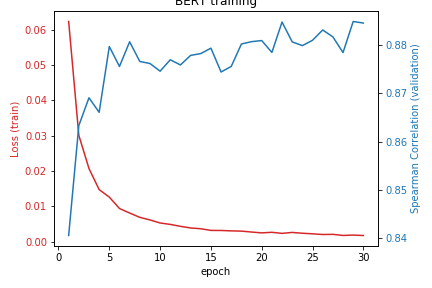
\includegraphics[width=\linewidth]{resources/bert-training.png}
  \caption{BERT fine-tuning over 13 epochs}
  \label{fig:bert:finetunning}
\end{figure}

\paragraph{Resultats} On obtient, avec BERT, un score très élevé, avec une corrélation sur les données de test de .877 (table \ref{table:models:results}).

%
\subsubsection{RoBERTa}

\paragraph{Hugging Face} Nous avons ensuite cherché à fine-tuner RoBERTa, version améliorée de BERT, en utilisant encore une fois la librairie transformers(\cite{huggingface}).

\paragraph{Training} Nous avons donc fine-tuné RoBERTa, en l'entrainant cette fois sur 10 époques, avec des batches de taille 8. Comme on peut le voire figure \ref{fig:bert:finetunning}, il suffit d'une (TODO) d'époques pour fine-tuner correctement le modèle. Cela nous prends, sur 1GPU, environ 30 minutes (table \ref{table:models:results}).

\begin{figure}
  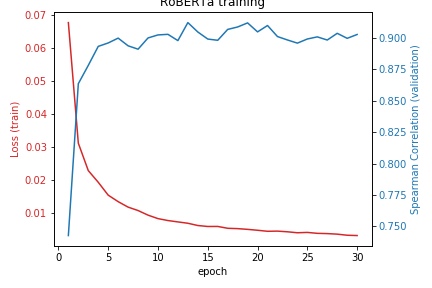
\includegraphics[width=\linewidth]{resources/roberta-training.png}
  \caption{ROBERTA fine-tuning over 10 epochs}
  \label{fig:roberta:finetunning}
\end{figure}

\paragraph{Resultats} On obtient, avec RoBERTa, un score légèrement meilleur que pour BERT, avec une corrélation sur les données de test de .891 (table \ref{table:models:results}), soit un gain de .014 par rapport à BERT.

%
\subsubsection{XLNet}

\paragraph{Hugging Face} Nous avons ensuite cherché à fine-tuner XLNet en utilisant à nouveau la librairie transformers(\cite{huggingface}).

\paragraph{Training} Nous avons donc fine-tuné XLNet, en l'entrainant sur X époques. Comme on peut le voire figure \ref{fig:xlnet:finetunning}, il suffit d'une (TODO) d'époques pour fine-tuner correctement le modèle. Cela nous prends, sur 1GPU, plus de 2h (table \ref{table:models:results}), XLNet étant beaucoup plus gros que BERT et RoBERTa.

\begin{figure}
  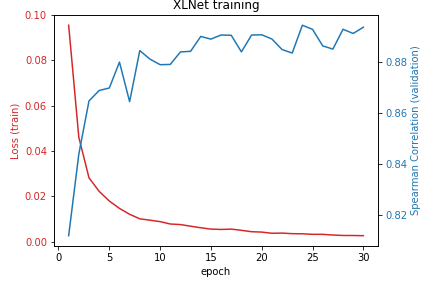
\includegraphics[width=\linewidth]{resources/xlnet-training.png}
  \caption{XLNet fine-tuning over 10 epochs}
  \label{fig:xlnet:finetunning}
\end{figure}

\paragraph{Resultats} On obtient, avec XLNet, un score similaire à celui de BERT, avec une corrélation de 0.884 (table \ref{table:models:results}) sur l'ensemble de test. Nous pensons que la taille du modèle le rends plus complexe à entraîner, mais qu'il pourrait avoir plus de potentiel si on l'entrainait plus longtemps, et avec plus de données.

%
\subsubsection{Moyenne des modeles}

Maintenant que nous avons 3 modèles très performants, issus du state-of-the-art, nous avons essayé de faire la moyenne des prédictions de ses modèles. Nous obtenons alors (table \ref{table:models:results}) d'excellents résultats, avec une corrélation de spearman sur l'ensemble de test de 0.906, ce qui nous fait gagner 0.015 points par rapport à RoBERTa, sur la corrélation de Spearman. On soulèvera que le défault de cette méthode est le temps de training (il faut entrainer les 3 modeles SOTA précédents), la taille des 3 modèles, et le temps d'inférence (il faut faire passer les phrases par chacun des 3 sous modèles).

%
\subsubsection{Stacking}

Nous avons ensuite essayé d'entrainer un modèle de réseaux de neuronnes fast-forward, avec une couche cachée de 16 neuronnes, à prédire la bonne valeur d'après les sorties des 3 sous modèles.

Pour ce faire, nous avons coupé le dataset d'entrainement en 3: 90\% du set étant utilisé pour fine-tuner séparément les 3 models SOTA, 90\% des données restantes (qu'aucun des 3 sous models n'a donc jamais vu) pour entrainer le model de stacking, le reste étant utilisé comme set de validation.

Nous obtenons de très bons résultats (table \ref{table:models:results}) sur les données de tests, avec une corrélation de spearman de 0.903. On remarque que ce score est plus grand que celui de validation: c'est parce qu'on a gardé très peu de données de validation. On aurait pu en prendre plus, mais au détriment soit de l'entrainement des sous modèles, soit de celui de stacking. Etant donné qu'il nous était possible de tester notre performance sur les données de test, nous n'avons pas jugé utile de le faire.

Nous avons ensuite essayé de changer la répartition des données entre l'entrainement des sous modèles et le stacking, pour passer à un 70\%-30\%. Cela n'a pas amélioré les résultats (table \ref{table:models:results}), confirmant notre hypothèse qu'il ne faut pas beaucoup de données pour entrainer le stacking, mais qu'il en faut beaucoup pour fine-tuner les sous modèles.

\begin{figure}
  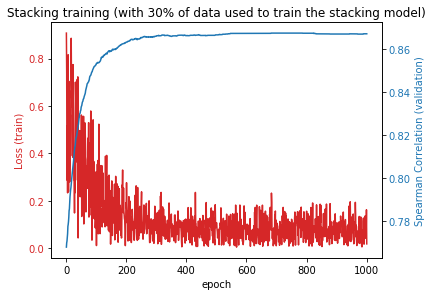
\includegraphics[width=\linewidth]{resources/stack-30-training.png}
  \caption{Entrainement du modèle de stacking sur 1000 époques}
  \label{fig:stack:train}
\end{figure}

\subsection{Discussion}


\section{Travaux connexes}



\section{Travaux futurs et conclusion }

%
\subsubsection{Travaux futurs}

Une piste qui pourrait etre envisagée, mais que nous n'avons pas pu essayer, est d'utiliser les dernières couches cachées des 3 sous models pour entrainer le modèle de stacking, au lieu de leur sortie (Fig.\ref{fig:stacking:archi_future}). On peut initialiser les poids de départ du réseau en concatenant ceux des sous modeles utilises, divises par le nombre de sous modeles (eq \ref{eq:stacking:future}); ainsi, le modele commence par predire la moyenne des sous modeles.

\begin{equation}
  h \leftarrow [h_{BERT} h_{RoBERTa} h_{XLNet}] / 3 \label{eq:stacking:future}
\end{equation}

\begin{figure}
\begin{center}
\begin{tikzpicture}[
  font=\sffamily,
  every matrix/.style={ampersand replacement=\&,column sep=.2cm,row sep=.3cm},
  layer/.style={draw,thick,rounded corners,fill=gray!3},
  data/.style={draw,shape=datastore,inner sep=.3cm},
  output/.style={draw,thick,circle,fill=green!20},
  model/.style={draw,very thick,fill=gray!20},
  dots/.style={gray,scale=2},
  to/.style={->,>=stealth',shorten >=1pt,semithick,font=\sffamily\footnotesize},
  every node/.style={align=center,inner sep=.2cm}]

  % Position the nodes using a matrix layout
  \matrix{
    \& \node[output] (score) {s}; \& \\

    \& \& \& \\
    \& \& \& \\

    \& \node[data] (features) {f11 | ... | f3x}; \& \node {(concatenation)}; \\

    \& \& \& \\
    \& \& \& \\

    \node[model] (bert) {BERT};  \& \node[model] (roberta) {RoBERTa}; \& \node[model] (xlnet) {XLNet}; \\

    \& \& \& \\

    \& \node[data] (sentences) {input sentences}; \& \\
  };

  % Draw the arrows between the nodes and label them.
  \draw[to] (features) -- node[midway,left] {
  \textbf{h}} (score);

  \draw[to] (bert) -- node[midway,left] {f11 | ... | f1b} (features);
  \draw[to] (roberta) -- node[midway,middle] {f21 | ... | f2r} (features);
  \draw[to] (xlnet) -- node[midway,right] {f31 | ... | f3x} (features);

  \draw[to] (sentences) -- (bert);
  \draw[to] (sentences) -- (roberta);
  \draw[to] (sentences) -- (xlnet);
\end{tikzpicture}
\caption{Architecture du modèle de stacking sur les dernières couches cachées} \label{fig:stacking:archi_future}
\end{center}
\end{figure}

\section*{Acknowledgments}
 

%where \verb|naaclhlt2019| corresponds to a naaclhlt2019.bib file.
\bibliography{naaclhlt2019}
\bibliographystyle{acl_natbib}

\appendix





\end{document}
